\documentclass[a4paper,11pt,twoside]{article}
\usepackage[utf8]{inputenc}	% Text coding
\usepackage[T1]{fontenc}
\usepackage{lmodern}
\usepackage[czech]{babel}
\usepackage{epsfig}
\usepackage{amsfonts,amsmath,amssymb}
\usepackage{graphicx}
\usepackage[unicode]{hyperref}
\usepackage{indentfirst}
\usepackage{fancyhdr}
\usepackage{xifthen}
\usepackage{amsthm,thmtools}
\usepackage{bold-extra}
\usepackage[dvipsnames]{xcolor}
\usepackage[subrefformat=simple,labelformat=simple]{subcaption} % Instead of subfigure
\usepackage{listings}
\usepackage{comment}
\usepackage{titlesec}
\usepackage{underscore}
\usepackage{makecell}       % Šířky čar v tabulkách

% Page size
\addtolength{\topmargin}{-1.5cm} %\addtolength{\textheight}{-10cm}
\addtolength{\textwidth}{4cm} \addtolength{\textheight}{4cm} % Width and height of the text
\addtolength{\voffset}{-0.5cm} % Top margin
\addtolength{\hoffset}{-2cm}
\setlength{\headheight}{15pt}

\DeclareMathOperator{\e}{e}

\def\vector#1{\boldsymbol{#1}}								% Vector
\renewcommand{\d}{\mathrm{d}}
\newcommand{\derivative}[3][]{\ifthenelse{\isempty{#1}}	    % Normal derivative
	{\frac{\d{#2}}{\d{#3}}}
	{\frac{\d^{#1}{#2}}{\d{#3}^{#1}}}
}
\newcommand{\im}{\mathrm{i}}

\def\makematrix#1{\begin{pmatrix}#1\end{pmatrix}}       % Matrix
\def\abs#1{\left|#1\right|}
\def\probability#1{\mathrm{Pr}\left[#1\right]}
\def\expectation#1{\mathrm{E}\left[#1\right]}
\def\dispersion#1{\sigma_{#1}^{2}}
\def\c{,\!}

\def\code#1{\textnormal{\texttt{#1}}}
\def\file#1{\textnormal{\textbf{\texttt{#1}}}}
\def\ghfile#1#2{\textnormal{\textbf{\texttt{\href{https://github.com/PavelStransky/PCInPhysics2021/blob/main/#1#2}{#2}}}}}

\def\abbreviation#1{\textnormal{\textsc{#1}}}

\begin{document}

\section*{Domácí úkol na 23.3.2022}
\subsection*{Lineární urychlovač}
Urychlovače v jaderné a částicové fyzice slouží k urychlování nabitých částic, například elektronů, protonů, ale i iontů těžších prvků.
Nejjednodušší lineární urychlovač sestává z periodicky se střídajících válců s dvěma rozdílnými potenciály $\varphi_{+}$ a $\varphi_{-}$:
\begin{center}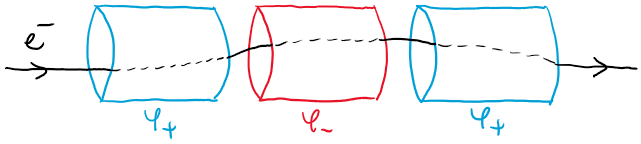
\includegraphics[width=0.7\linewidth]{accelerator.png}\end{center}
My se pro jednoduchost omezíme na dvourozměrný model:
\begin{center}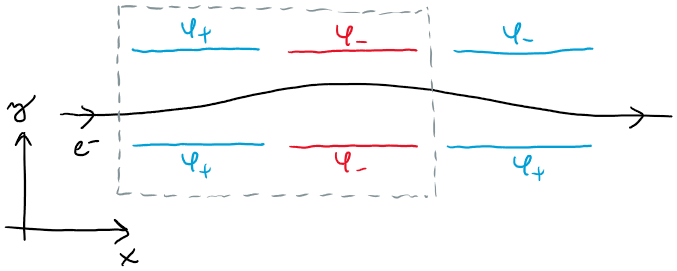
\includegraphics[width=0.7\linewidth]{accelerator2D.png}\end{center}
Pokud do urychlovače vpustíme nabitou částici s dostatečnou rychlostí a přibližně na ose mezi horní a dolní elektrodou, její rychlost ve směru $x$ se bude postupně zvyšovat.
Zařízení bude zároveň svazek udržovat v okolí osy.

\begin{enumerate}
    \item Modifikujte kód ze cvičení pro řešení dvourozměrné Poissonovy rovnice a implementujte \emph{periodickou okrajovou podmínku} ve směru osy $x$.
    
    \item S periodickou okrajovou podmínkou spočítejte elektrostatický potenciál pro jeden segment urychlovače zobrazený na obrázku šedivým čárkovaným obdélníkem.
        Periodická okrajová podmínka v tomto případě simuluje nekonečně dlouhý urychlovač.
    
    \item Spočítejte intenzitu elektrického pole $\vector{E}=-\nabla{\varphi}$ v každém bodě mříže.
    
    \item Spočítejte trajektorii nabité částice, kterou do zařízení vystřelíte s počáteční rychlostí $\vector{v}_{0}=(v_{0x},v_{0y})$.
        Využijte znalost numerického řešení obyčejných diferenciálních rovnic z prvních dvou cvičení.
    
    \item Zakreslete závislost longitudinální rychlosti částice na čase $v_{x}(t)$.
\end{enumerate}

Uvažujte jednotky $\epsilon_{0}=1,e=1$. 
Vzdálenost desek volte 20 jednotek, délku desek 50 jednotek. 
Mezi deskami s kladným potenciálem $\varphi_{+}=+1$ a záporným potenciálem $\varphi_{+}=-1$ jsou 2 jednotky mezera.
Počáteční poloha elektronu v čase $t_{0}=0$ je na začátku první desky 2 jednotky od osy zařízení, počáteční rychlost je $v_{x0}=20, v_{y0}=0$.
Spočítejte trajektorii do času $t=200$.

Více informací o urychlování nabitých částic najdete například \href{http://ipnp.cz/~dolejsi/textbook/Accelerators_CZ.ppt}{v prezentaci doc. Jiřího Dolejšího}.

Vypracovaný úkol odešlete na e-mailovou adresu \href{mailto:pcfyzika@pavelstransky.cz}{pcfyzika@pavelstransky.cz}.
Před odesláním se přesvědčte, že program neobsahuje žádné syntaktické chyby a že je z kódu pochopitelné, jak ho spustit, aby vrátil hledaný výsledek.
\end{document}